\documentclass[10pt,landscape]{article}
\usepackage{multicol}
\usepackage{calc}
\usepackage[landscape]{geometry}
\usepackage{amsmath,amsthm,amsfonts,amssymb,relsize}
\usepackage{color,graphicx,overpic}

% Turn off header and footer
\pagestyle{empty}
\geometry{top=.25in,left=.25in,right=.25in,bottom=.25in}

% Redefine section commands to use less space
\makeatletter
\renewcommand{\section}{\@startsection{section}{1}{\z@}{3ex}{2ex}
                       {\normalfont\normalsize\bfseries\textit}}
\renewcommand{\subsection}{\@startsection{subsection}{2}{\z@}{2ex}{0.5ex}
                          {\normalfont\small\bfseries}}
\makeatother

% Don't print section numbers
\setcounter{secnumdepth}{0}

\setlength{\parindent}{0pt}
\setlength{\parskip}{0pt}

\newcommand{\R}{\mathbb{R}}
\newcommand{\E}{\mathbb{E}}

\newcommand{\ba}{\mathbf{a}}
\newcommand{\bb}{\mathbf{b}}
\newcommand{\bv}{\mathbf{v}}
\newcommand{\bx}{\mathbf{x}}
\newcommand{\by}{\mathbf{y}}
\newcommand{\bz}{\mathbf{z}}

\newcommand{\bA}{\mathbf{A}}
\newcommand{\bB}{\mathbf{B}}
\newcommand{\bH}{\mathbf{H}}
\newcommand{\bI}{\mathbf{I}}
\newcommand{\bJ}{\mathbf{J}}
\newcommand{\bW}{\mathbf{W}}
\newcommand{\bX}{\mathbf{X}}
\newcommand{\bY}{\mathbf{Y}}
\newcommand{\bZ}{\mathbf{Z}}

\newcommand{\bhy}{\hat{\mathbf{y}}}

\newcommand{\balpha}{\boldsymbol{\alpha}}
\newcommand{\bbeta}{\boldsymbol{\beta}}
\newcommand{\bdelta}{\boldsymbol{\delta}}
\newcommand{\btheta}{\boldsymbol{\theta}}
\newcommand{\bmu}{\boldsymbol{\mu}}
\newcommand{\bxi}{\boldsymbol{\xi}}
\newcommand{\bSigma}{\boldsymbol{\Sigma}}
\newcommand{\bLambda}{\boldsymbol{\Lambda}}

\newcommand{\diag}{\text{diag}}
\newcommand{\tp}[1]{#1^{\prime}}
\newcommand{\inv}[1]{#1^{-1}}
\newcommand{\norm}[1]{\|#1\|}
\newcommand{\gaussian}[2]{\mathcal{N}(#1, #2)}
\newcommand{\inR}[2]{#1 \in \R^{#2}}
\newcommand{\dfi}[1]{f^{\prime(#1)}}
\newcommand{\pfrac}[2]{\frac{\partial #1}{\partial #2}}
\newcommand{\ruler}{\\\rule{\columnwidth}{0.25pt}\\}

% For neural net.
\newcommand{\la}[2]{#1^{(#2)}}
\newcommand{\nbs}{n^{bs}}

% -----------------------------------------------------------------------
\begin{document}
\raggedright
\footnotesize
\begin{multicols*}{3}
% multicol parameters
% These lengths are set only within the two main columns
% \setlength{\columnseprule}{0.1pt}
\setlength{\premulticols}{1pt}
\setlength{\postmulticols}{1pt}
\setlength{\multicolsep}{1pt}
\setlength{\columnsep}{0pt}

\section{Module 6: Iterators and Joins}
\textbf{Iterators}:\\
setup(), init(), next(), close()\\
useful because it streams data and therefore does not have to use a lot of memory or space to access large amounts of data that might not fit into memory
\ruler
\textbf{Cost Notation for Join Analysis}:\\
$[R]$: the number of pages to store R\\
$p_R$: the number of records per page of R\\
$|R|$: the cardinality (number of records) of R (=$[R] \cdot p_R$)
\ruler
\textbf{Variants of Nested Loop Join}:\\
\textit{Simple}: $[R] + |R|[S]$\\
We can change join order to lower cost.\\
for each record $r$ in R do\\
\-\hspace{0.5cm} for each record $s$ in S do\\
\-\hspace{1cm} if $\theta(r,s)$, then add $<r,s>$ to result buffer\\
\textit{Page}: $[R] + [R][S]$\\
We can operate at granularity of pages rather than tuples\\
for each rpage in R:\\
\-\hspace{0.5cm} for each spage in S:\\
\-\hspace{1cm} for each rtuple in rpage:\\
\-\hspace{1.5cm} for each stuple in spage:\\
\-\hspace{2.0cm} if $\theta(rtupe, stuple)$:\\
\-\hspace{2.5cm} add $<rtuple, stuple>$ to result buffer\\
\textit{Block}: $[R] + \lceil\frac{[R]}{B-2}\rceil[S]$\\
We can extend granularity to blocks of pages.\\
for each rchunk of B-2 pages of R\\
\-\hspace{0.5cm} for each spage of S:\\
\-\hspace{1.0cm} for all matching tuples in spage and rchunk:\\
\-\hspace{1.5cm} add $<rtuple, stuple>$ to result buffer
\ruler
\textbf{Index Nested Join Loop}:\\
We join one data table with another data table that is indexed on a B+ tree.\\
for each rtuple in R:\\
\-\hspace{0.5cm} for each stuple in S where rtuple == stuple:\\
\-\hspace{1.0cm} add $<rtuple, stuple>$ to result\\
If index uses Alt. 1, the  cost is just that to traverse tree from root to leaf. For Alt. 2 and 3, the total cost is the sum between the cost to look up the record id (tree height) plus the cost to retrieve the record having found the record id. The retrieval cost is 1 I/O per page of matching S tuples if the index is clustered; if index is unclustered, 1 I/O per matching S tuple. \\
\textit{Unclustered Cost(R, S)} = $[R] + |R| \cdot (\text{num matching stuples for each rtuple}) \cdot (\text{access cost per stuple})$.
\textit{Clustered Cost(R, S)} = $[R] + |R| \cdot (\text{num matching spages for each rtuple}) \cdot (\text{access cost per spage})$.
\ruler
\textbf{Sort Merge Join}:\\
1) Sort tuples in R and S by join key\\
2) Merge-scan the sorted partitions and output matches\\
if (!mark)\\
\-\hspace{0.5cm} while (r $<$ s) advance r \\
\-\hspace{0.5cm} while (r $>$ s) advance s \\
\-\hspace{0.5cm} mark = s // mark start of "block" of S \\
if (r == s) \\
\-\hspace{0.5cm} result = $<$ r, s $>$\\
\-\hspace{0.5cm} advance s\\
\-\hspace{0.5cm} yield result\\
else\\
\-\hspace{0.5cm} reset s to mark\\
\-\hspace{0.5cm} advance r\\
\-\hspace{0.5cm} mark = NULL\\
\textit{average cost} = sort R + sort S + ($[$R$]$ + $[$S$]$)
\ruler
\textbf{Grace Hash Join}\\
1) Partition tuples from R and S by join key and store on disk.\\
2) Build + Probe a separate hash table for each partition.\\
for relation Cur in {R, S} // stage 1\\ 
\-\hspace{0.5cm} for page in Cur\\
\-\hspace{1.0cm} read page into input buffer\\
\-\hspace{1.0cm} for tuple on page\\
\-\hspace{1.5cm} place tuple in output buf hash$_p$(tuple.joinkey)\\
\-\hspace{1.5cm} if output buf full, flush to disk partition\\
\-\hspace{0.5cm} flush remaining output bufs to disc partitions\\
for $i$ in $[0...(B-1)]$\\
\-\hspace{0.5cm} for page in $R_i$\\
\-\hspace{1.0cm} for tuple on page\\
\-\hspace{1.5cm} build tuple into memory hash$_r$ (tuple.joinkey)\\
\-\hspace{0.5cm} for page in $S_i$\\
\-\hspace{1.0cm} read page into input buffer\\
\-\hspace{1.0cm} for tuple on page\\
\-\hspace{1.5cm} prob memory hash$_r$ for matches\\
\-\hspace{1.5cm} send all matches to output buffer\\
\-\hspace{1.5cm} flush output buffer if full\\

% --------------------------------

\section{Module 7: Query Optimization}
\textbf{Common Heuristics}\\
Apply \textit{selections} as long as you have the relative columns.\\
\textit{Project} unnecessary columns away as soon as we can, so extra data does not get copied or moved around unnecessarily.\\
We want to minimize \textit{cartesian products} since they are very costly.\\
Selection can be cascaded and is commutative.
\ruler
\textbf{Physical Equivalences}\\
\textit{Base Table Access}: heap scan and index scan.\\
\textit{Equijoin}: Block Nested Loop for simple operations that exploit extra memory, Index Nested Loop is effective if 1 table is relatively small and the other is indexed properly, Sort-Merge Join is good with small memory, equal-size tables, Grace Hash Join is even better than sort if the tables are differently sized.\\
\textit{Non-Equijoins}: Block Nested Loop is the only option, as the others are designed for finding matches.

% --------------------------------

\section{Module 8: Transactions and Concurrency}
\textbf{Definition and Advantages}\\
Multiple transactions are allowed to run concurrently in the system. Increased processor/disk utilization means greater \textit{throughput} (transactions per second), and one transaction's \textit{latency} (response time per transaction) is not dependent on another unrelated transaction.\ruler
\textbf{Lost Update}: Two users update the record at the same time. \textbf{Inconsistent Read}: User reads in the middle of another user's transaction which is not a state intended by either user.\\ \textbf{Dirty Read}: A user updates the record while another user reads the record.
\ruler
\textbf{Atomicity}: All actions in the Xact happen, or none happen. DBMS should ensure that updates of a partially executed transaction are not reflected.
\ruler
\textbf{Consistency}: If the DB starts out consistent, it ends up consistent at the end of Xact (primary key constraints, type constraints, or functional dependencies like foreign keys).
\ruler
\textbf{Isolation}: Execution of each Xact is isolated from that of others. Each Xact executes as if it ran by itself. The net effect should be identical to executing all transactions in some serial order.
\ruler
\textbf{Durability}: If a Xact commits, effects persist. Any commits not yet sent to disk must survive any failures or system crashes.
\ruler
DBMS typically ensures \textit{atomicity} and \textit{durability} by \textit{loggingg} all actions: it undoes the actions of failed/aborted transactions and redoes actions of committed transactions not yet propagated to disk when the system crashes.
\ruler
\textbf{Transaction Schedule}: A sequence of actions on data from one or more transactions. Actions include Begin, Read, Write, Commit, and Abort. By convention, we only include committed transactions and omit Begin and Commit.
\ruler
\textbf{Serial Equivalence / Serializability}: 2 schedules are equivalent if they involve the same transactions, each indivdual transaction's actions are ordered the same, and both schedules leave the DB in the same final state. We want to find an optimal schedule that is equivalent to a \textit{serial} schedule where each transaction runs from start to finish without any intervening actions from other transactions.
\ruler
Two operations \textbf{conflict} when they 1) are by different transactions, 2) are on the same resource, and 3) at least one of them is a write.
\ruler
Two schedules are \textbf{conflict equivalent} iff they involve the same actions of the same transactions and every pair of conflicting actions is ordered the same way.
\ruler
Schedule S is \textbf{conflict serializable} if S is conflict equivalent to some serial schedule. This implies S is also serializable. However, note that some serializable schedules are not cconflict serializable. So when we test if a schedule is conflict serializable, we may produce false negatives for whether it is also serializable. This is the cost of a conservative, yet highly more efficient, test. We can transform S into a a serial schedule by swapping consecutive non-confliting operations of different transactions.
\ruler
\textbf{Conflict Dependency Graph}: There is one node per Xact. There exists an edge from $T_i$ to $T_j$ if an operation $O_i$ conflicts with an operation $O_j$ and $O_i$ appears earlier in the schedule than $O_j$. The schedule is conflict serializable iff its dependency graph is acyclic.
\ruler
\textbf{View Serializability}: An alternative notion of serializability that offers fewer false negatives. Schedules S1 and S2 are view equivalent if:\\
1) \textit{Same initial reads}: If $T_i$ reads initial value of A in S1, then $T_i$ also reads initial value of A in S2.\\
2) \textit{Same dependent reads}: If $T_i$  reads value of A written by $T_j$ is S1, then $T_i$ also reads value of A written by $T_j$ in S2.\\
3) \textit{Same winning writes}: If $T_i$ writes final value of A in S1, then $T_i$ also writes final value of A in S2.
\ruler
\textbf{Two Phase Locking (2PL)}: Most common scheme for enforcing conflict serializability; Considered "pessimistic" - will set locks on resources for fear of conflict; this pessimism induces some cost; An Xact must obtain a S (shared) lock before reading and an X (exclusive) lock before writing.
\ruler
2PL \textbf{acquires} and \textbf{releases}. A transaction cannot acquire any new locks after it begins releasing locks (this point is the "lock point"). Lock points guarantee conflict serializability because at these points, transactions have everything they need locked and any other conflicting transactions either started their release phase before this point or are blocked waiting for this transaction.
\ruler
\textbf{Cascading Aborts}: The abort/rollback of one transaction requires abort/rollback of another transaction. Example: $R_1(A), W_1(A), R_2(A), W_2(A), Abort_1$.
\ruler
\textbf{Strict 2PL}: Same as 2PL, but only when a transaction completes (either commits all writes or aborts and undoes all writes) does it release all its locks (thereby avoiding cascading aborts)
\ruler
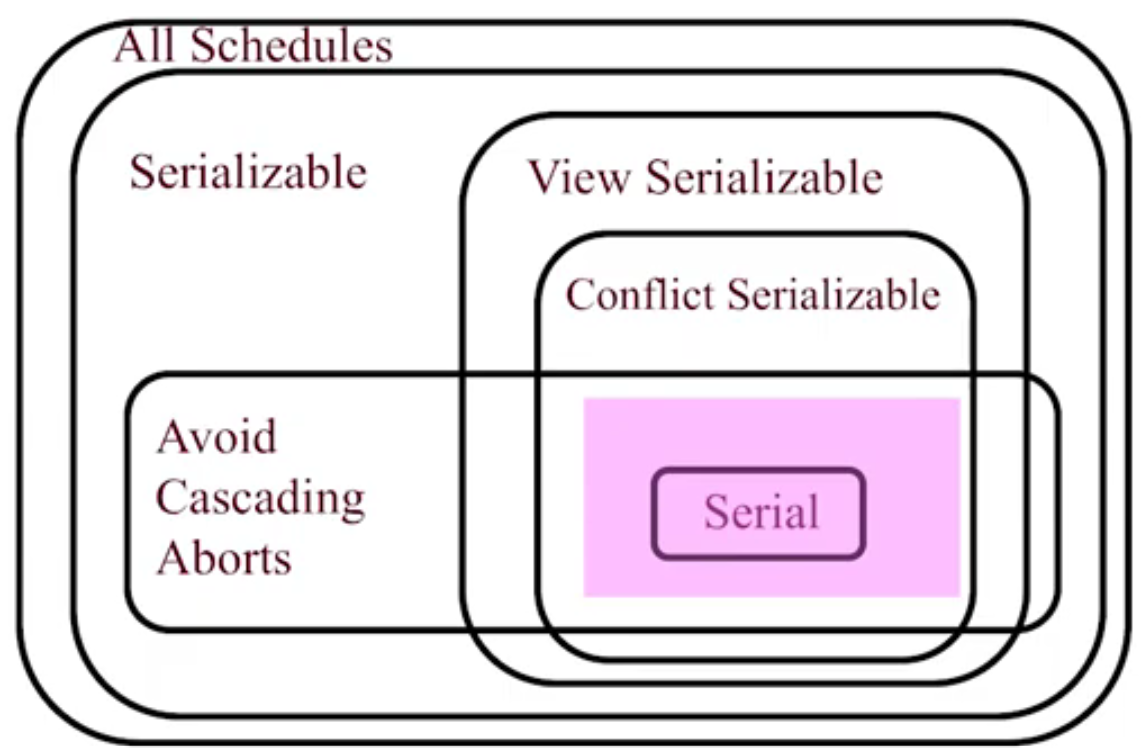
\includegraphics[width=0.25\textwidth]{images/SerializabiltySchedulePIcture.png}
\ruler
\textbf{Lock Management}: When lock request arrives, it either a) does not conflict with locks held by other transactions and is put in the granted set or b) does conflict and is put into the wait queue (FIFO).
\ruler
\textbf{Deadlock}: A cycle of Xacts waiting for locks to be released for each other. 
\ruler
We can \textbf{avoid deadlocks} with two approaches: Given $T_i$ wants a lock that $T_j$ holds, 1) \textit{Wait-Die}: if $T_i$ has higher priority, $T_i$ waits for $T_j$; else $T_i$ aborts; 2) \textit{Wound-Wait}: 1) if $T_i$ has higher priority, $T_j$ aborts; else $T_i$ waits
\ruler
Deadlock avoidance succeeds b/c the same priority scheme applies on all lock conflicts, DBMSs can safely roll back transactions, and higher-priority transactions eventually get access.
\ruler
\textbf{Deadlock Detection and Waits-For Graph}: An arrow from a $T_i$ node to a $T_j$ node signifies $T_i$ waits for $T_j$, and a cycle in the graph means a deadlock exists. A DBMS will periodically extract a waits-for graph, find cycles, and abort one of the deadlocked transaction on the cycle.
\ruler
\textbf{Additional Lock Modes}: \textbf{IS}: Intent to get S lock(s) at finer granularity, \textbf{IX}: Intent to get X lock(s) at finer granularity, \textbf{SIX}: S and IX at teh same time
\ruler
\textbf{Multigranularity Locking Protocol}: To get S or IS lock on a node, must hold IS or IX on parent node; to get X or IX or SIX on a node, must hold IX or SIX on parent node; must release locks in bottom-up order
\ruler
\textbf{Compatibility Between Locks}:\\
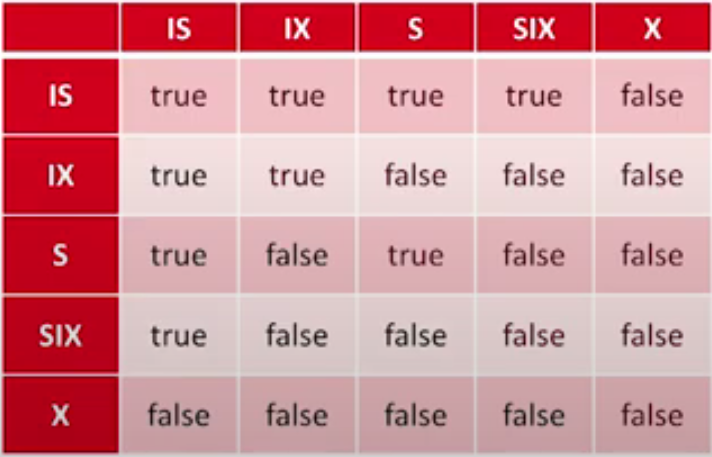
\includegraphics[width=0.2\textwidth]{images/CompatibilityMatrix.png}
\section{Module 9: Recovery}
\textbf{Sources of Aborted Xacts} 1) User explicitly issues rollback; 2) Deadlock; 3) System crash; 4) Consistency, i.e. integrity constraint violation
\ruler
\textbf{Sources of DBMS Crashes} 1) Operator Error; 2) Configuration Error; 3) Soft/Hardware failure
\ruler
\textbf{Force / No Force}: Ensures durability; When a Xact has finished, \textit{Force} pushes all modified data pages to disk before the Xact commits. Could be unnecessary because since other Xacts likely also are modifying the in-memory page, we write to disk repeatedly; \textit{No-Force} writes to disk only when the page needs to be evicted from the buffer pool; complicates durability; if DB  crashes after transaction commits, dirty pages may not been written to disk and are lost from memory but will be resolved by redoing operations during recovery.
\ruler
\textbf{Steal / No Steal}: Ensures atomicity; \textit{No-Steal} does not allow pages to be evicted from memory (written to disk and saved) until the Xact commits; \textit{Steal} allows modified pages to be written to disk before a Xact finishes; the DB can \textit{steal} pages before a Xact has even finished; complicates atomicity the DB is left in an intermediate state) but will be resolved by undoing bad operations during recovery.
\ruler
\textbf{ARIES - Analysis}: Rebuild what the Xact Table and the Dirty Page Table looked like at the time of the crash. Scan all log records from the start.\\
1. On any record that is not an END record: add the Xact to the Xact Table (if necessary). Set the lastLSN of the Xact to the LSN of the record you are on.\\
2. If the record is a COMMIT or an ABORT record, change the status of the Xact in the Xact table accordingly.\\
3. If the record is an UPDATE record, if the page is not in the DPT add the page to the DPT and set recLSN equal to the LSN.\\
4. If the record is an END record, remove the Xact from the Xact Table.
\ruler
\textbf{Checkpointing}: Writes the contents of the Xact Table and the DPT to the log in order to speed up the analysis phase. Rather than starting at the beginning of the log when we analyze, we can start at the last checkpoint. Writes two records to the log, a $<BEGINCHECKPOINT>$ record and an $<ENDCHECKPOINT>$ record that says when we finished writing the tables to the log.
\ruler
\textbf{ARIES - Redo}: Ensures durability. Starts at the smallest recLSN in the DPT b/c that is the first op that may not have made it to disk. Will redo all UPDATE and CLR ops unless one of the following conditions is met:\\
\-\hspace{0.5cm} 1. The page is not in the DPT. If the page is not in the DPT, it implies that all changes have already been flushed to disk.\\
\-\hspace{0.5cm} 2. recLSN $\geq$ LSN. The first update that dirtied the page occurred after this operation. Implies that the operation we are currently at has already made it to disk, other wise it woudl be the recLSN.\\
\-\hspace{0.5cm} 3. pageLSN (disk) $\geq$ LSN. If the most recent update to the page that made it to disk occurred after the current operation, then we know the current operation must have made it to disk.
\ruler
\textbf{ARIES - Undo}: Ensures atomicity; starts at the end of the log; undoes every UPDATE for each Xact that was active (running/aborting) at the time of the crash so we do not leave the state in an intermediate state. Will not undo UPDATE if it already has been undone and has a CLR record already in the log for that UPDATE. For every UPDATE undone, we write a corresponding CLR record to the log. It will have an additional field, undoNextLSN, that stores the LSn of the next operation to be undone for that Xact (coming from the prevLSN of the operation that is being undone). Once all undoing operations for a Xact are completed, write the END record for that Xact to the log.

\section{Module 10: Database Design}

\section{Module 11: Parallel Query Processing}
\section{Module 12: Distributed Transactions}
\section{Module 13: Non-Relational Data Models and NoSQL}
\section{Module 14: MapReduce and Spark}
\end{multicols*}
\end{document}